% Options for packages loaded elsewhere
\PassOptionsToPackage{unicode}{hyperref}
\PassOptionsToPackage{hyphens}{url}
%
\documentclass[
  english,
  man,floatsintext]{apa6}
\usepackage{lmodern}
\usepackage{amsmath}
\usepackage{ifxetex,ifluatex}
\ifnum 0\ifxetex 1\fi\ifluatex 1\fi=0 % if pdftex
  \usepackage[T1]{fontenc}
  \usepackage[utf8]{inputenc}
  \usepackage{textcomp} % provide euro and other symbols
  \usepackage{amssymb}
\else % if luatex or xetex
  \usepackage{unicode-math}
  \defaultfontfeatures{Scale=MatchLowercase}
  \defaultfontfeatures[\rmfamily]{Ligatures=TeX,Scale=1}
\fi
% Use upquote if available, for straight quotes in verbatim environments
\IfFileExists{upquote.sty}{\usepackage{upquote}}{}
\IfFileExists{microtype.sty}{% use microtype if available
  \usepackage[]{microtype}
  \UseMicrotypeSet[protrusion]{basicmath} % disable protrusion for tt fonts
}{}
\makeatletter
\@ifundefined{KOMAClassName}{% if non-KOMA class
  \IfFileExists{parskip.sty}{%
    \usepackage{parskip}
  }{% else
    \setlength{\parindent}{0pt}
    \setlength{\parskip}{6pt plus 2pt minus 1pt}}
}{% if KOMA class
  \KOMAoptions{parskip=half}}
\makeatother
\usepackage{xcolor}
\IfFileExists{xurl.sty}{\usepackage{xurl}}{} % add URL line breaks if available
\IfFileExists{bookmark.sty}{\usepackage{bookmark}}{\usepackage{hyperref}}
\hypersetup{
  pdftitle={The acceptability of two reflexives in one clause: identity, blocking and dialectual variations},
  pdfauthor={Chaoyi Chen},
  pdflang={en-EN},
  pdfkeywords={keywords},
  hidelinks,
  pdfcreator={LaTeX via pandoc}}
\urlstyle{same} % disable monospaced font for URLs
\usepackage{graphicx}
\makeatletter
\def\maxwidth{\ifdim\Gin@nat@width>\linewidth\linewidth\else\Gin@nat@width\fi}
\def\maxheight{\ifdim\Gin@nat@height>\textheight\textheight\else\Gin@nat@height\fi}
\makeatother
% Scale images if necessary, so that they will not overflow the page
% margins by default, and it is still possible to overwrite the defaults
% using explicit options in \includegraphics[width, height, ...]{}
\setkeys{Gin}{width=\maxwidth,height=\maxheight,keepaspectratio}
% Set default figure placement to htbp
\makeatletter
\def\fps@figure{htbp}
\makeatother
\setlength{\emergencystretch}{3em} % prevent overfull lines
\providecommand{\tightlist}{%
  \setlength{\itemsep}{0pt}\setlength{\parskip}{0pt}}
\setcounter{secnumdepth}{-\maxdimen} % remove section numbering
% Make \paragraph and \subparagraph free-standing
\ifx\paragraph\undefined\else
  \let\oldparagraph\paragraph
  \renewcommand{\paragraph}[1]{\oldparagraph{#1}\mbox{}}
\fi
\ifx\subparagraph\undefined\else
  \let\oldsubparagraph\subparagraph
  \renewcommand{\subparagraph}[1]{\oldsubparagraph{#1}\mbox{}}
\fi
% Manuscript styling
\usepackage{upgreek}
\captionsetup{font=singlespacing,justification=justified}

% Table formatting
\usepackage{longtable}
\usepackage{lscape}
% \usepackage[counterclockwise]{rotating}   % Landscape page setup for large tables
\usepackage{multirow}		% Table styling
\usepackage{tabularx}		% Control Column width
\usepackage[flushleft]{threeparttable}	% Allows for three part tables with a specified notes section
\usepackage{threeparttablex}            % Lets threeparttable work with longtable

% Create new environments so endfloat can handle them
% \newenvironment{ltable}
%   {\begin{landscape}\begin{center}\begin{threeparttable}}
%   {\end{threeparttable}\end{center}\end{landscape}}
\newenvironment{lltable}{\begin{landscape}\begin{center}\begin{ThreePartTable}}{\end{ThreePartTable}\end{center}\end{landscape}}

% Enables adjusting longtable caption width to table width
% Solution found at http://golatex.de/longtable-mit-caption-so-breit-wie-die-tabelle-t15767.html
\makeatletter
\newcommand\LastLTentrywidth{1em}
\newlength\longtablewidth
\setlength{\longtablewidth}{1in}
\newcommand{\getlongtablewidth}{\begingroup \ifcsname LT@\roman{LT@tables}\endcsname \global\longtablewidth=0pt \renewcommand{\LT@entry}[2]{\global\advance\longtablewidth by ##2\relax\gdef\LastLTentrywidth{##2}}\@nameuse{LT@\roman{LT@tables}} \fi \endgroup}

% \setlength{\parindent}{0.5in}
% \setlength{\parskip}{0pt plus 0pt minus 0pt}

% Overwrite redefinition of paragraph and subparagraph by the default LaTeX template
% See https://github.com/crsh/papaja/issues/292
\makeatletter
\renewcommand{\paragraph}{\@startsection{paragraph}{4}{\parindent}%
  {0\baselineskip \@plus 0.2ex \@minus 0.2ex}%
  {-1em}%
  {\normalfont\normalsize\bfseries\itshape\typesectitle}}

\renewcommand{\subparagraph}[1]{\@startsection{subparagraph}{5}{1em}%
  {0\baselineskip \@plus 0.2ex \@minus 0.2ex}%
  {-\z@\relax}%
  {\normalfont\normalsize\itshape\hspace{\parindent}{#1}\textit{\addperi}}{\relax}}
\makeatother

% \usepackage{etoolbox}
\makeatletter
\patchcmd{\HyOrg@maketitle}
  {\section{\normalfont\normalsize\abstractname}}
  {\section*{\normalfont\normalsize\abstractname}}
  {}{\typeout{Failed to patch abstract.}}
\patchcmd{\HyOrg@maketitle}
  {\section{\protect\normalfont{\@title}}}
  {\section*{\protect\normalfont{\@title}}}
  {}{\typeout{Failed to patch title.}}
\makeatother
\shorttitle{The acceptability of two reflexives in one clause}
\keywords{keywords\newline\indent Word count: X}
\usepackage{csquotes}
\usepackage{float}
\floatplacement{figure}{H}
\ifxetex
  % Load polyglossia as late as possible: uses bidi with RTL langages (e.g. Hebrew, Arabic)
  \usepackage{polyglossia}
  \setmainlanguage[]{english}
\else
  \usepackage[shorthands=off,main=english]{babel}
\fi
\ifluatex
  \usepackage{selnolig}  % disable illegal ligatures
\fi
\newlength{\cslhangindent}
\setlength{\cslhangindent}{1.5em}
\newlength{\csllabelwidth}
\setlength{\csllabelwidth}{3em}
\newenvironment{CSLReferences}[2] % #1 hanging-ident, #2 entry spacing
 {% don't indent paragraphs
  \setlength{\parindent}{0pt}
  % turn on hanging indent if param 1 is 1
  \ifodd #1 \everypar{\setlength{\hangindent}{\cslhangindent}}\ignorespaces\fi
  % set entry spacing
  \ifnum #2 > 0
  \setlength{\parskip}{#2\baselineskip}
  \fi
 }%
 {}
\usepackage{calc}
\newcommand{\CSLBlock}[1]{#1\hfill\break}
\newcommand{\CSLLeftMargin}[1]{\parbox[t]{\csllabelwidth}{#1}}
\newcommand{\CSLRightInline}[1]{\parbox[t]{\linewidth - \csllabelwidth}{#1}\break}
\newcommand{\CSLIndent}[1]{\hspace{\cslhangindent}#1}

\title{The acceptability of two reflexives in one clause: identity, blocking and dialectual variations}
\author{Chaoyi Chen\textsuperscript{}}
\date{}


\affiliation{\vspace{0.5cm}\textsuperscript{1} Rutgers University}

\begin{document}
\maketitle

\hypertarget{methods}{%
\section{Methods}\label{methods}}

Mandarin has two kinds of reflexives: the simple reflexive \emph{ziji} `self' and the complex reflexive \emph{ta-ziji} `him-self.' When appearing in a subordinate clause, both \emph{ziji} and \emph{ta-ziji} can refer to the subject in the matrix clause. For example, in the sentence `\emph{John} thinks that \emph{ziji}/\emph{ta-ziji} is clever,' both \emph{ziji} and \emph{ta-ziji}' are able to refer to the matrix subject \emph{John}. This paper examines the case where two reflexives appears in one subordinate clause and explores the factors affecting the acceptability of the sentence. In the sentence `\emph{John} thinks that REF1 cheats REF2.' REF1 and REF2 can be occupied by either \emph{ziji} or \emph{ta-ziji}, thus four possibilities are generated: \emph{ziji}-\emph{ziji}, \emph{ta-ziji}-\emph{ta-ziji}, \emph{ziji}-\emph{ta-ziji} and \emph{ta-ziji}-\emph{ziji}. On top of these four cases, three factors of theoretical interests are considered in this study: (i) whether or not two reflexives are identical; (ii) whether or not a less specific reflexive precedes a more specific reflexive (\emph{ziji}-\emph{ta-ziji} vs the other three cases; I called the cases of a less specific reflexive preceding a more specific reflexive as \textbf{blocking} hereafter); (iii) whether or not the speaker is a northern Mandarin speaker. This is a hypothetical project and the data were stimulated by the R-package \emph{faux}.

\hypertarget{participants}{%
\subsection{Participants}\label{participants}}

This study recruited a total of 100 participants, among which 50 participant were northern Mandarin speakers and 50 participants were southern Mandarin speakers (non-northern Mandarin speakers). Their northern/southern identities are defined in term of the dialects they speak. Participants were screened such that their age were greater than 18 years old.

\hypertarget{procedure}{%
\subsection{Procedure}\label{procedure}}

Participants completed the tests individually and finished the following tasks in order: a consent form (5 minutes), a language background questionnaire (5 minutes), an acceptability rating task (15 minutes).

\hypertarget{language-background-questionnaire}{%
\subsection{Language background questionnaire}\label{language-background-questionnaire}}

It was administered in the participants' L1 (Mandarin) and contained the questions about the dialect(s) they speak, the age of acquisition of Mandarin, knowledge of other languages, and language experience and use.

\hypertarget{materials}{%
\subsection{Materials}\label{materials}}

This study tested four sentences in total. These four sentences is framed as \emph{Zhangsan} thinks that REF1 cheats REF2. The four sentences for test instantiate the four possibilities of reflexive combinations: \emph{ziji}-\emph{ziji}, \emph{ta-ziji}-\emph{ta-ziji}, \emph{ziji}-\emph{ta-ziji} and \emph{ta-ziji}-\emph{ziji}. For the identity variable, \emph{ziji}-\emph{ziji}, \emph{ta-ziji}-\emph{ta-ziji} are marked as yes and \emph{ziji}-\emph{ta-ziji} and \emph{ta-ziji}-\emph{ziji} are marked as no. For the blocking parameter, \emph{ziji}-\emph{ziji}, \emph{ta-ziji}-\emph{ta-ziji}and \emph{ta-ziji}-\emph{ziji} are marked as yes while \emph{ziji}-\emph{ta-ziji} is marked as no.

\hypertarget{the-acceptability-rating-task}{%
\subsection{The acceptability rating task}\label{the-acceptability-rating-task}}

This experiment was an acceptability rating task administered online using XXX, a data collecting website. Sentence items were presented one at a time which participants rated on a scale from 1 (very bad) to 7 (very good) intuitively as a formal measure of linguistic acceptability. These Likert scales have been widely used in psychological research (Likert 1932; Hartley 2014) as well as judgment replication studies. Participants were required to judge the acceptability of 20 sentences: 8 practice sentences and 12 non-practice sentences (8 fillers, 4 experimental). A one-minute break was placed after the first ten sentences were rated. The practice sentences served to familiarize subjects with the task and 7-point rating system. The order of items presented in the experiment was randomized.

\hypertarget{results}{%
\section{Results}\label{results}}

\hypertarget{data-summary}{%
\subsection{Data summary}\label{data-summary}}

We obtained 400 observations in total from 100 participants and each participant rated on four test sentences. The sentence of four combinations \emph{ziji}-\emph{ta-ziji}, \emph{ta-ziji}-\emph{ziji}, \emph{ziji}-\emph{ziji} and \emph{ta-ziji}-\emph{ta-ziji} were marked as ``s1,''``s2,''``s3'' and ``s4'' respectively in the raw data and their identity and blocking properties were added to the data frame after the experiment (a part of data cleaning). The data frame for analysis is shown below. The participant from S001 to S050 are northern Mandarin speakers and the participant from S051-S100 are Mandarin Chinese speakers.

\begin{table}
\centering
\begin{tabular}{l|l|l|r|l|l}
\hline
id & dia & sentence & rating & Blocking & Identity\\
\hline
S001 & nor & s1 & 1 & yes & no\\
\hline
S001 & nor & s2 & 1 & no & no\\
\hline
S001 & nor & s3 & 4 & no & yes\\
\hline
S001 & nor & s4 & 5 & no & yes\\
\hline
S002 & nor & s1 & 2 & yes & no\\
\hline
S002 & nor & s2 & 3 & no & no\\
\hline
\end{tabular}
\end{table}

\hypertarget{descriptive-statistics}{%
\subsection{Descriptive statistics}\label{descriptive-statistics}}

The descriptive statistics of acceptability ratings (mean, standard deviation(SD) and the number of observations) for the four sentences are given in the table below. The acceptability ratings with respect to blocking, identity and dialectual background are presented in Fig.1, Fig.2 and Fig.3 respectively.

\begin{table}

\centering
\begin{tabular}[t]{l|l|l|r}
\hline
Blocking & mean & SD & N\\
\hline
no & 4.693 & 2.033 & 300\\
\hline
yes & 3.38 & 2.206 & 100\\
\hline
\end{tabular}
\centering
\begin{tabular}[t]{l|l|l|r}
\hline
Identity & mean & SD & N\\
\hline
no & 3.66 & 2.151 & 200\\
\hline
yes & 5.07 & 1.911 & 200\\
\hline
\end{tabular}
\centering
\begin{tabular}[t]{l|l|l|r}
\hline
dia & mean & SD & N\\
\hline
nor & 2.575 & 1.328 & 200\\
\hline
sou & 6.155 & 1.037 & 200\\
\hline
\end{tabular}
\end{table}

The overall pattern suggest that the sentences without blocking (mean = 4.69; SD = 2.03) have higher scores than the sentences with blocking (mean = 3.38; SD = 2.21); the sentences with identical reflexives (mean = 5.07; SD = 1.91) have higher scores than the sentences with different reflexives (mean = 3.66; SD = 2.15); the acceptability rating of the sentences in question is lower for northern Mandarin speakers (mean = 2.58; SD = 1.33) than southern Mandarin speakers (mean = 6.16; SD = 1.04).

\begin{figure}

{\centering 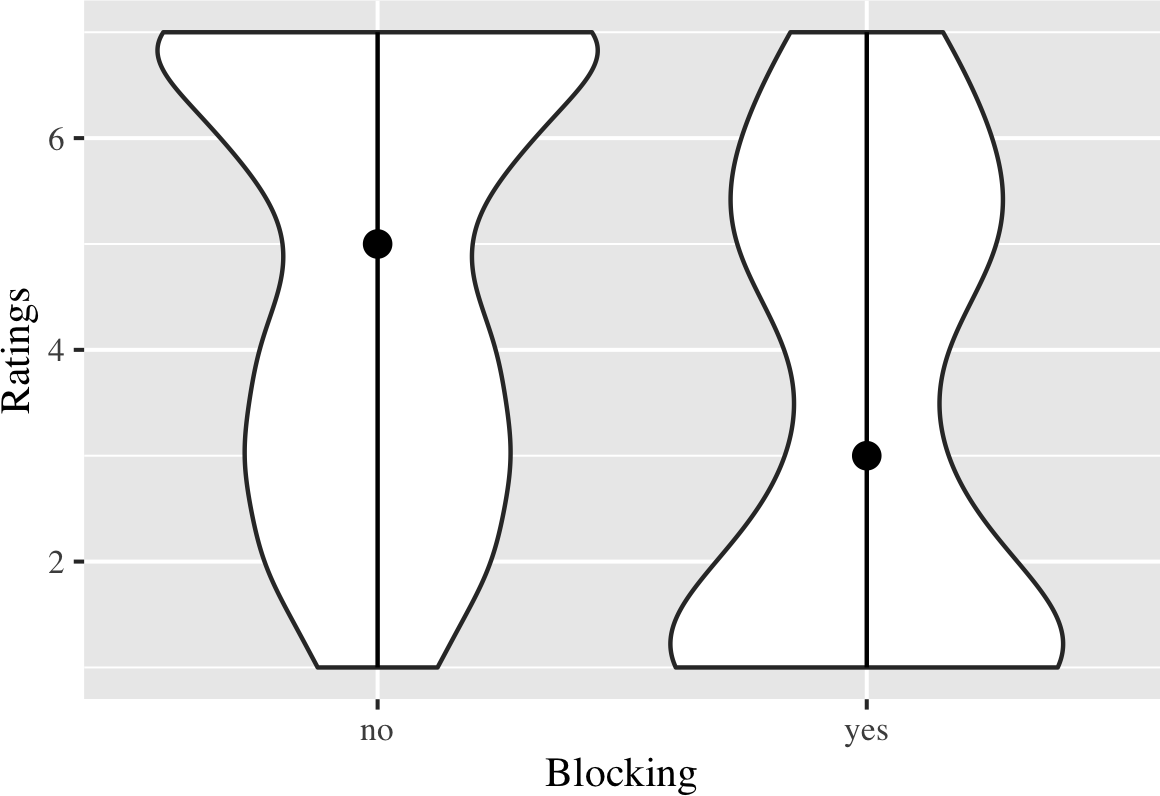
\includegraphics{manuscript_files/figure-latex/plot11-1} 

}

\caption{The ratings of blocking and non-blocking sentences}\label{fig:plot11}
\end{figure}

\begin{figure}

{\centering 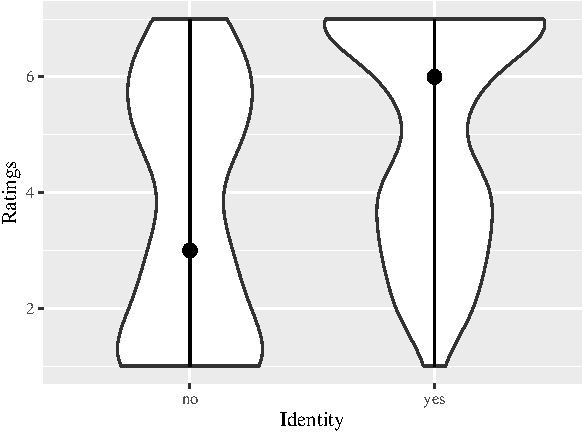
\includegraphics{manuscript_files/figure-latex/plot12-1} 

}

\caption{The ratings of identical and non-identical sentences}\label{fig:plot12}
\end{figure}
\begin{figure}

{\centering 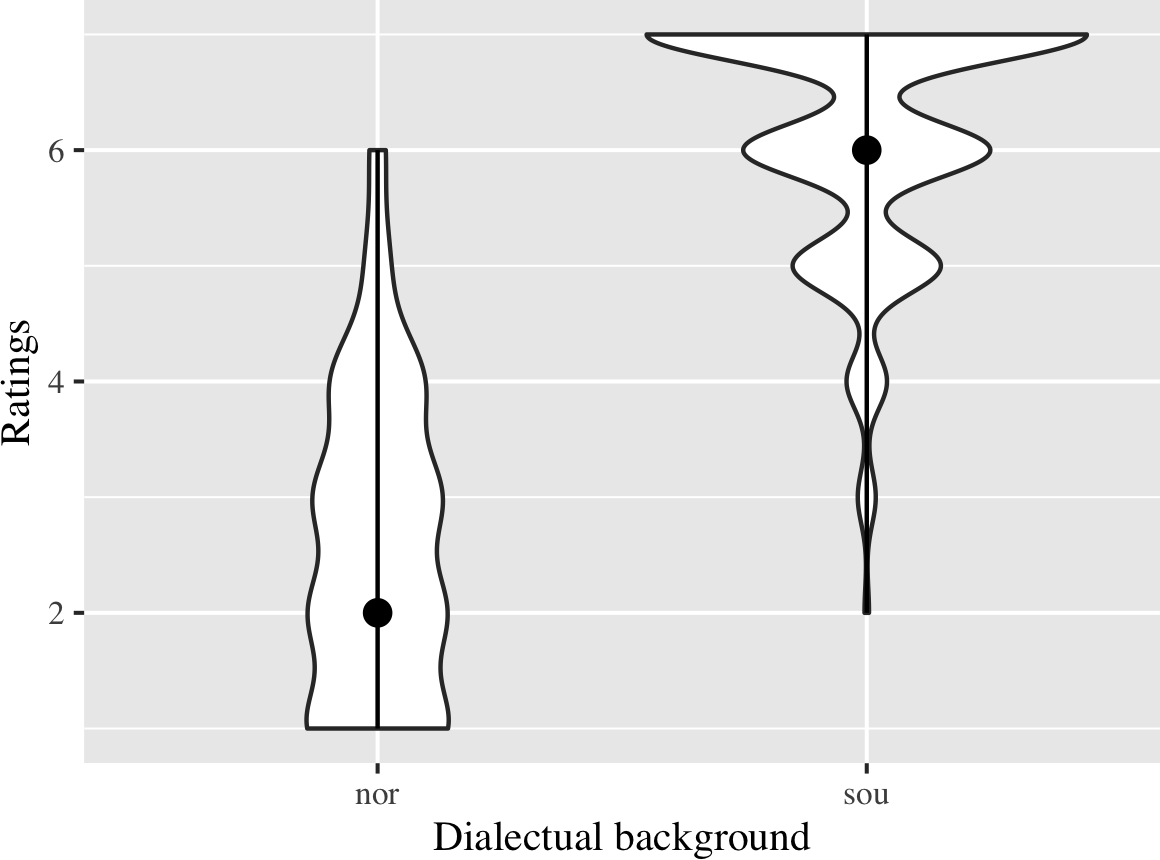
\includegraphics{manuscript_files/figure-latex/plot13-1} 

}

\caption{The ratings from northern and northern participants}\label{fig:plot13}
\end{figure}

The ratings by individuals are presented in Fig 4. The participants S001-S050, who are northern Mandarin speakers (the left side of the table) have lower ratings in general than the participants S051-S100, who are southern Mandarin speakers (the right side of the table).

\begin{figure}

{\centering 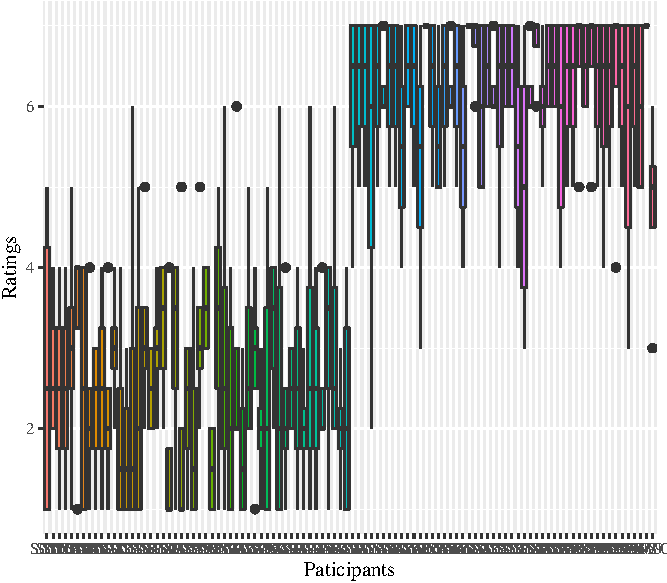
\includegraphics{manuscript_files/figure-latex/plot14-1} 

}

\caption{Individual Ratings from northern and southern participants}\label{fig:plot14}
\end{figure}

\hypertarget{cumulative-link-mixed-model}{%
\subsection{Cumulative link mixed model}\label{cumulative-link-mixed-model}}

Due to the ordinal nature of the outcome variable, this study used cumulative link mixed model (CLMM) to analyze the rating score data, and experiment-wise alpha was set at 0.05. The categorical fixed effect group was dummy coded with no (for Blocking), yes (for Identity) and northern speaker (for dialectual background) set as the baseline. The random effects structure only included by-subject random intercepts because the predictors are independent from each other. A total of five models were fitted: fm1 (only including intercept), fm2 (including the predictor Blocking), fm3 (including the predictor Blocking and Identity), fm4 (including the predictor Blocking, Identity and dialectual background) and fm5 (including the predictor Blocking, Identity and dialectual background as fixed effects and the random effects of subject). The comparison of these five models are given below.

\begin{tabular}{l|r|r|r|r|r|r}
\hline
  & no.par & AIC & logLik & LR.stat & df & Pr(>Chisq)\\
\hline
fm1 & 6 & 1535 & -762 & NA & NA & NA\\
\hline
fm2 & 7 & 1505 & -746 & 31.68 & 1 & 0.000\\
\hline
fm3 & 8 & 1486 & -735 & 21.77 & 1 & 0.000\\
\hline
fm4 & 9 & 963 & -473 & 524.18 & 1 & 0.000\\
\hline
fm5 & 10 & 964 & -472 & 1.28 & 1 & 0.257\\
\hline
\end{tabular}

As a result, the model containing Blocking, Identity and dialectual background (fm4) had the lowest AIC value (1486) and thus provided the best fit of the data as shown in the table below. Blocking (z = -4.18, p \textless{} 0.001), Identity (z = 8.95, p \textless{} 0.001) and dialectual background (z = 16.76, p \textless{} 0.001) all have main effects on the final rating scores. Given the data from fm5, we are not confident enough to conclude that the random effect of participants show a main effect in this study (p = 0.257 \textgreater{} 0.05).

\begin{tabular}{l|r|r|r|r|l}
\hline
term & estimate & std.error & statistic & p.value & coef.type\\
\hline
1|2 & -0.645 & 0.239 & -2.70 & 0.007 & intercept\\
\hline
2|3 & 1.002 & 0.235 & 4.26 & 0.000 & intercept\\
\hline
3|4 & 2.471 & 0.267 & 9.25 & 0.000 & intercept\\
\hline
4|5 & 3.987 & 0.327 & 12.19 & 0.000 & intercept\\
\hline
5|6 & 5.477 & 0.389 & 14.10 & 0.000 & intercept\\
\hline
6|7 & 7.371 & 0.455 & 16.21 & 0.000 & intercept\\
\hline
Blockingyes & -1.138 & 0.272 & -4.18 & 0.000 & location\\
\hline
Identityyes & 2.283 & 0.255 & 8.95 & 0.000 & location\\
\hline
diasou & 6.367 & 0.380 & 16.76 & 0.000 & location\\
\hline
\end{tabular}

\newpage

\hypertarget{references}{%
\section{References}\label{references}}

\begingroup
\setlength{\parindent}{-0.5in}
\setlength{\leftskip}{0.5in}

\hypertarget{refs}{}
\begin{CSLReferences}{1}{0}
\leavevmode\hypertarget{ref-hartley2014some}{}%
Hartley, J. (2014). Some thoughts on likert-type scales. \emph{International Journal of Clinical and Health Psychology}, \emph{14}(1), 83--86.

\leavevmode\hypertarget{ref-likert1932technique}{}%
Likert, R. (1932). A technique for the measurement of attitudes. \emph{Archives of Psychology}.

\leavevmode\hypertarget{ref-R-base}{}%
R Core Team. (2021). \emph{R: A language and environment for statistical computing}. Vienna, Austria: R Foundation for Statistical Computing. Retrieved from \url{https://www.R-project.org/}

\end{CSLReferences}

\endgroup


\end{document}
